
%%%%%%%%%%%%%%%%%%%%%%%%%%%%%%%%%%%%%%%%%%%%%%%%%%%%%%%%%%%%%%%%%%%%%%%%%%%%%%%%
%%%%%%%%%%% Document class and package options
%%%%%%%%%%%%%%%%%%%%%%%%%%%%%%%%%%%%%%%%%%%%%%%%%%%%%%%%%%%%%%%%%%%%%%%%%%%%%%%%
% \documentclass[a4paper,12pt]{article}
\documentclass[a4paper,12pt,twoside]{article}
\usepackage{outline}

\usepackage{amsmath}
\usepackage{amssymb}                    % AMS Math
\usepackage{amsfonts}
\usepackage[tight,hang,centerlast]{subfigure}
\usepackage[lined,ruled,longend]{algorithm2e}
\usepackage{longtable}
\usepackage{verbatim}

%\usepackage[dvipsnames]{xcolor}

\usepackage{rotating}

\usepackage{fancyvrb}




\clubpenalty=1000
\widowpenalty=1000

%% eps to pdf
%% specify .eps extension when \includegraphics if you want the .pdf fig file to
%%     be regenerated as part of the compilation. Without extension the .pdf fig
%%     file is generated only if it does not exist yet
%% --shell-escape option must be enabled
\newif\ifpdf
\ifx\pdfoutput\undefined
   \pdffalse
\else
   \pdfoutput=1
   \pdftrue
\fi
\ifpdf
   \usepackage{graphicx}
   \usepackage{epstopdf}

   \epstopdfsetup{suffix=}

   \DeclareGraphicsRule{.eps}{pdf}{.pdf}{`epstopdf #1}
   \pdfcompresslevel=9
\else
   \usepackage{graphicx}
\fi

% redefine \VerbatimInput
\RecustomVerbatimCommand{\VerbatimInput}{VerbatimInput}%
{fontsize=\tiny,
 %
 frame=lines,  % top and bottom rule only
 framesep=2em, % separation between frame and text
% rulecolor=\color{Gray},
 %
 label=\fbox{ping.stat},
 labelposition=topline,
 %
 commandchars=\|\(\), % escape character and argument delimiters for
                      % commands within the verbatim
 commentchar=*        % comment character
}

\begin{document}


%%%%%%%%%%%%%%%%%%%%%%%%%%%%%%%%%%%%%%%%%%%%%%%%%%%%%%%%%%%%%%%%%%%%%%%%%%%%%%%%
%%%%%%%%%%% Title
%%%%%%%%%%%%%%%%%%%%%%%%%%%%%%%%%%%%%%%%%%%%%%%%%%%%%%%%%%%%%%%%%%%%%%%%%%%%%%%%

\title{Measurement Results from\\
Wireless Battle Mesh\\
Version 7}


%\date{Mai, 2014}

\contributors{WBM community}
\eventlocation{Sublab. Leipzig, Germany}
\eventdates{12th to 18th of May 2014}
\eventurl{http://battlemesh.org/BattleMeshV7}
\doctype{Measurement Analysis (work in progress)}
\logofigure{figures/battlemeshv7}

\frontmatter

\maketitle

%%%%%%%%%%%%%%%%%%%%%%%%%%%%%%%%%%%%%%%%%%%%%%%%%%%%%%%%%%%%%%%%%%%%%%%%%%%%%%%%
%%%%%%%%%%% Indices
%%%%%%%%%%%%%%%%%%%%%%%%%%%%%%%%%%%%%%%%%%%%%%%%%%%%%%%%%%%%%%%%%%%%%%%%%%%%%%%%

\thispagestyle{plain}
%\vspace*{3cm}

%\begin{center}
%\LARGE{\textbf{Abstract}} 
%\end{center}

%\begin{itemize}
%\item TODO..
%\end{itemize}

%\cleardoublepage
\clearsinglepage

\thispagestyle{plain}
\tableofcontents

%\cleardoublepage
\clearsinglepage

%%%%%%%%%%%%%%%%%%%%%%%%%%%%%%%%%%%%%%%%%%%%%%%%%%%%%%%%%%%%%%%%%%%%%%%%%%%%%%%%
%%%%%%%%%%% The document
%%%%%%%%%%%%%%%%%%%%%%%%%%%%%%%%%%%%%%%%%%%%%%%%%%%%%%%%%%%%%%%%%%%%%%%%%%%%%%%%

\singlespacing
\mainmatter
%%%%%%%%%%%%%%%%%%%%%%%%%%%%%%%%%%%%%%%%%%%%%%%%%%%%%%%%%%%%%%%%%%%%%%%%%%%%%%%%
%%%%%%%%%%% Chapter Inclusion
%%%%%%%%%%%%%%%%%%%%%%%%%%%%%%%%%%%%%%%%%%%%%%%%%%%%%%%%%%%%%%%%%%%%%%%%%%%%%%%%


%%%%%%%%%%%%%%%%%%%%%%%%%%%%%%%%%%%%%%%%%%%%%%%%%%%%%%%%%%%%%%%%%%%%%%%%%%%%%%%%
%%%%%%%%%%%%%%%%%%%%%%%%%%%%%%%%%%%%%%%%%%%%%%%%%%%%%%%%%%%%%%%%%%%%%%%%%%%%%%%%
\thispagestyle{plain}

%%%%%%%%%%%%%%%%%%%%%%%%%%%%%%%%%%%%%%%%%%%%%%%%%%%%%%%%%%%%%%%%%%%%%%%%%%%%%%%%
%%%%%%%%%%%%%%%%%%%%%%%%%%%%%%%%%%%%%%%%%%%%%%%%%%%%%%%%%%%%%%%%%%%%%%%%%%%%%%%%
%%%%%%%%%%%%%%%%%%%%%%%%%%%%%%%%%%%%%%%%%%%%%%%%%%%%%%%%%%%%%%%%%%%%%%%%%%%%%%%%
\section{Introduction}
\label{sec:introduction}


WBM...

%%%%%%%%%%%%%%%%%%%%%%%%%%%%%%%%%%%%%%%%%%%%%%%%%%%%%%%%%%%%%%%%%%%%%%%%%%%%%%%%
%%%%%%%%%%%%%%%%%%%%%%%%%%%%%%%%%%%%%%%%%%%%%%%%%%%%%%%%%%%%%%%%%%%%%%%%%%%%%%%%
%%%%%%%%%%%%%%%%%%%%%%%%%%%%%%%%%%%%%%%%%%%%%%%%%%%%%%%%%%%%%%%%%%%%%%%%%%%%%%%%
% A summary of protocol itself, the used versions and configuration

%\section{Protocols}


%\subsection{Babel}

%\subsection{Batman-adv}

%\subsection{Bmx6}

%\subsection{OLSR}

\section{Data and System Repositories}



\scriptsize
\begin{verbatim}
http://wibed.confine-project.eu

https://github.com/battlemesh/wibed (buildroot)
https://github.com/battlemesh/wibed-battlemesh-experiment (package)
http://wiki.confine-project.eu/wibed:start
https://github.com/axn/wbm2pdf  (this stuff, branch wbmv7 in future)

Raw measurement data:
http://wibed.confine-project.eu/resultsdir/wbmv7-axn-16_2014-05-16_19-28-43 (stationary scenarios)
http://wibed.confine-project.eu/resultsdir/wbmv7-axn-17_2014-05-16_20-13-20 (broken crossed streams scenario)
http://wibed.confine-project.eu/resultsdir/wbmv7-axn-19_2014-05-16_21-35-33 (mobile scenarios)

\end{verbatim}
\normalsize
%%%%%%%%%%%%%%%%%%%%%%%%%%%%%%%%%%%%%%%%%%%%%%%%%%%%%%%%%%%%%%%%%%%%%%%%%%%%%%%%
%%%%%%%%%%%%%%%%%%%%%%%%%%%%%%%%%%%%%%%%%%%%%%%%%%%%%%%%%%%%%%%%%%%%%%%%%%%%%%%%
%%%%%%%%%%%%%%%%%%%%%%%%%%%%%%%%%%%%%%%%%%%%%%%%%%%%%%%%%%%%%%%%%%%%%%%%%%%%%%%%
\section{Testbed Descripiton}

\subsection{Nodes and Locations}


\scriptsize
\begin{verbatim}
NodeID  Location               exp:axn-16   exp:axn-17  exp:axn-19
                               (stationary) (broken)    (mobile)
164a7a  deathroom
3b3a90  workshopRoom
3b3d70  ????
3e9db0  deathroom??            9db0->1ab0               9db0->4174
51aac8  halleAnfang                                     aac8->4174
8a417e  deathroom              417e->4174  417e->1ab0 
c24174  HalleEnde (mobile)                 4174->1936 
c2427a  deathroom??                                     427a->4174
ce3360  EloiTable
e4b63a  mustiTable
e60a62  halleMitte
e60aac  deathroom
e60ad6  deathroom
e61936  axelsTable             1936->4174  1936->4174   1936->4174
f41ab0  kloschiOffice??        1ab0->4174  1ab0->417e   1ab0->4174
\end{verbatim}
\normalsize


\subsection{Topology}

% wget http://downloads.battlemesh.org/WBMv6/geographical_map1.png
% wget http://downloads.battlemesh.org/WBMv6/geographical_map2.png
%\begin{figure}[!ht]
%\centering
%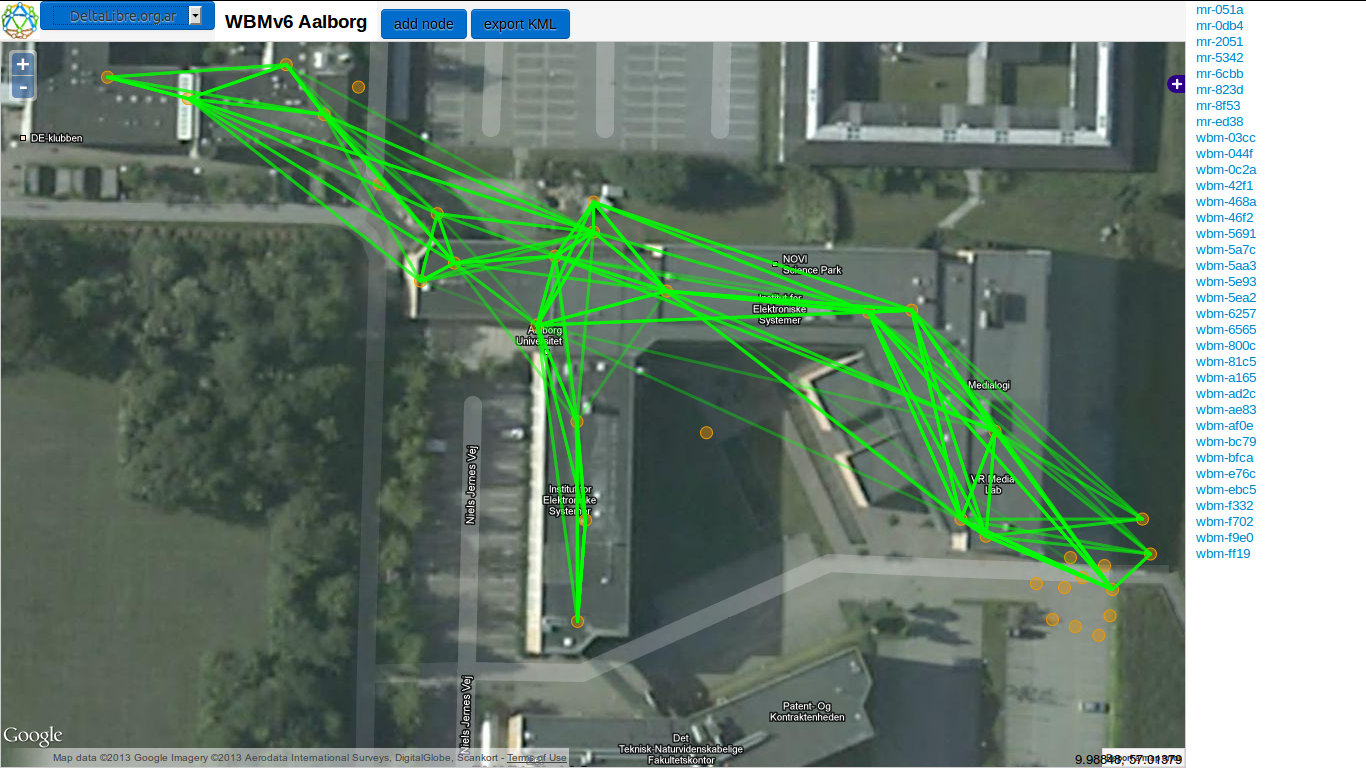
\includegraphics[width=1.4\textwidth, angle=90]{figures/geographical_map2.png}
%\caption{geographical map snapshot}
%\label{fig:geomap}
%\end{figure}


% wget -O topo0.svg "http://battlemesh.org/BattleMeshV6/Tests?action=AttachFile&do=get&target=topo0.svg"
% \immediate\write18{ inkscape -D -z --file=topo0.svg --export-pdf=topo0.pdf }

%\begin{figure}[!ht]
%\centering
%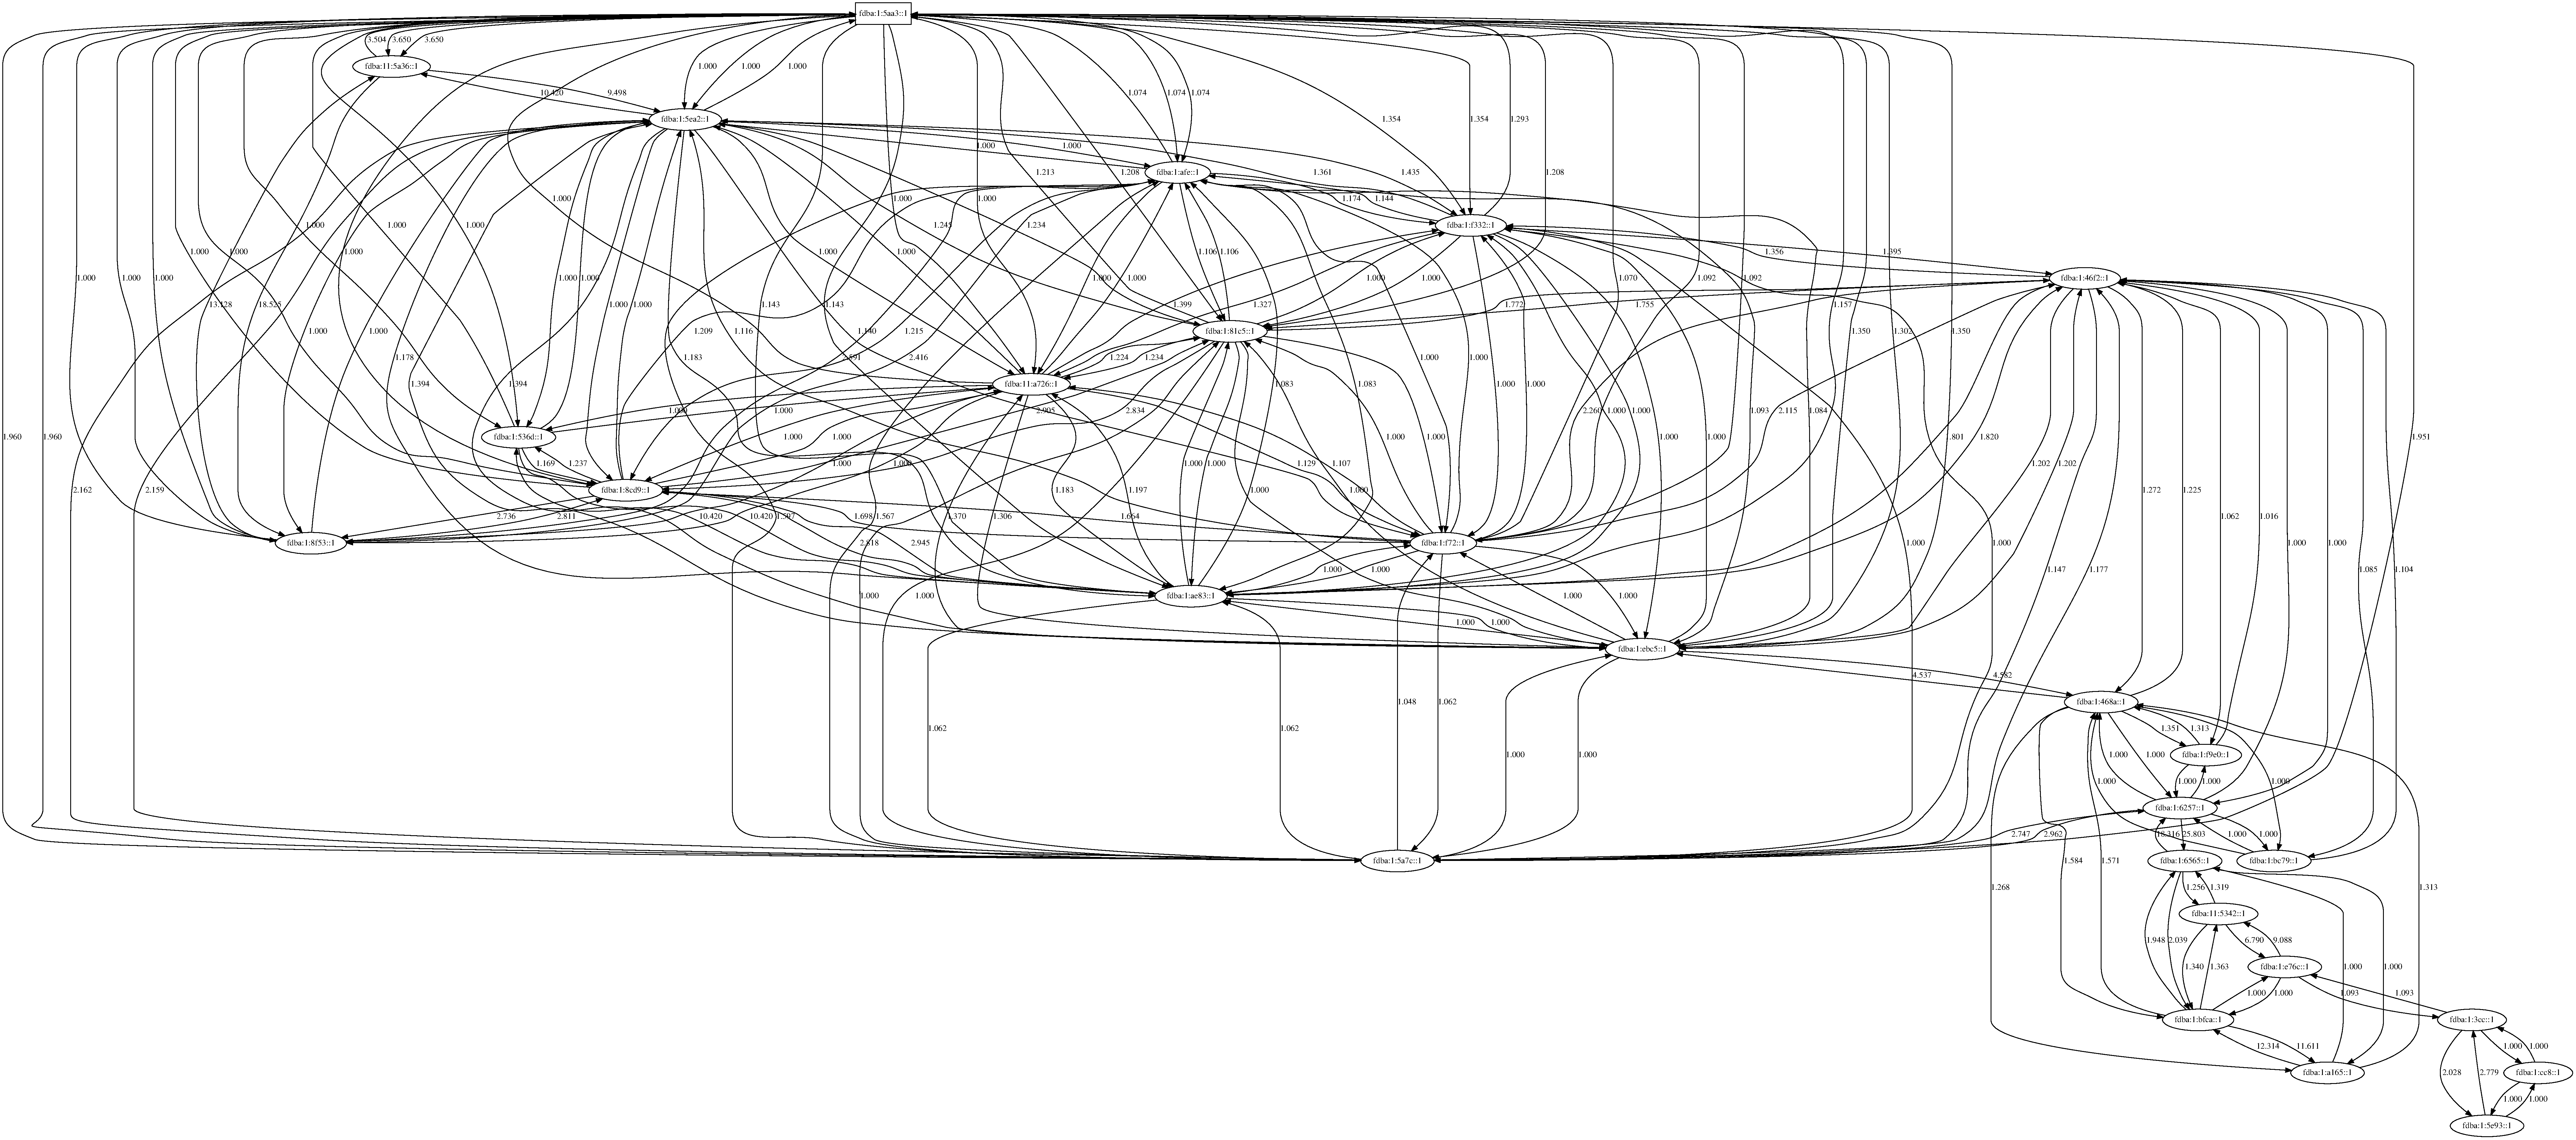
\includegraphics[width=1.4\textwidth, angle=90]{figures/topo0.pdf}
%\caption{OLSR topology snapshot}
%\label{fig:olsr-topo}
%\end{figure}

%\begin{figure}[h]
%\centering
%\def\svgwidth{\columnwidth}
%\includesvg{topo0}
%\end{figure}

\clearpage

%%%%%%%%%%%%%%%%%%%%%%%%%%%%%%%%%%%%%%%%%%%%%%%%%%%%%%%%%%%%%%%%%%%%%%%%%%%%%%%%
%%%%%%%%%%%%%%%%%%%%%%%%%%%%%%%%%%%%%%%%%%%%%%%%%%%%%%%%%%%%%%%%%%%%%%%%%%%%%%%%
%%%%%%%%%%%%%%%%%%%%%%%%%%%%%%%%%%%%%%%%%%%%%%%%%%%%%%%%%%%%%%%%%%%%%%%%%%%%%%%%
\section{Ping Measurements (hops, rtt, loss)}
\label{sec:ping-measurements}


%%%%%%%%%%%%%%%%%%%%%%%%%%%%%%%%%%%%%%%%%%%%%%%%%%%%%%%%%%%%%%%%%%%%%%%%%%%%%%%%
%\immediate\write18{ ../eval.R --data=../tmp.data --stat=../tmp.stat --imgdir=../img --texdir=inputs/ }

%%%%%%%%%%%%%%%%%%%%%%%%%%%%%%%%%%%%%%%%%%%%%%%%%%%%%%%%%%%%%%%%%%%%%%%%%%%%%%%%
\subsection{Stationary Scenarios}

\clearpage
%\makeFigure{sArtt}{Random node test 1}{0.69} 
%\makeFigure{sArvh}{Random node test 1}{0.69}

\clearpage

%\makeFigure{sBrtt}{Random node test 2}{0.69}
%\makeFigure{sBrvh}{Random node test 2}{0.69}


\clearpage


\subsection{Ping Results Table}

The folloing verbatim table lists statistics per experiment (EXP) and group (GRP) as calculated by the lua-based
evaluation script based on the raw ping-measurements data and outputted to the file ping.stat.
Event based results are given for each received icmp response in ping.data.


%\VerbatimInput{../ping.stat}

\subsection{Stationary Nodes Measurements}

\makeCCCTabl{tbl:p1}{End-to-end ping6 performance between two stationary nodes: 9db0-1ab0, 417e-4174, 1936-4174, 1ab0-4174} {%
%  \makeCCCPingGraphic{}
  \makeCCCPingGraphic{./test_data/wbmv7-axn-16_2014-05-16_19-28-43/wbmv7-axn-16_2014-05-16_19-28-43_wibed-3e9db0/wbm-axn}
  \makeCCCPingGraphic{./test_data/wbmv7-axn-16_2014-05-16_19-28-43/wbmv7-axn-16_2014-05-16_19-28-43_wibed-8a417e/wbm-axn}
  \makeCCCPingGraphic{./test_data/wbmv7-axn-16_2014-05-16_19-28-43/wbmv7-axn-16_2014-05-16_19-28-43_wibed-e61936/wbm-axn}
  \makeCCCPingGraphic{./test_data/wbmv7-axn-16_2014-05-16_19-28-43/wbmv7-axn-16_2014-05-16_19-28-43_wibed-f41ab0/wbm-axn}
}

%\makeCCCTabl{tbl:p2}{concurrent End-to-end ping6 performance between four stationary nodes 1936-4174 and 1ab0-417e} {%
%  \makeCCCPingGraphic{./test_data/wbmv7-axn-17_2014-05-16_20-13-20/wbmv7-axn-17_2014-05-16_20-13-20_wibed-e61936/wbm-axn}
%  \makeCCCPingGraphic{./test_data/wbmv7-axn-17_2014-05-16_20-13-20/wbmv7-axn-17_2014-05-16_20-13-20_wibed-f41ab0/wbm-axn}
%}

%\makeCCCTabl{tbl:p3}{concurrent End-to-end ping6 performance between four stationary nodes 417e-1ab0 and 4174-1926} {%
%  \makeCCCPingGraphic{./test_data/wbmv7-axn-17_2014-05-16_20-13-20/wbmv7-axn-17_2014-05-16_20-13-20_wibed-8a417e/wbm-axn} %broken daemons
%  \makeCCCPingGraphic{./test_data/wbmv7-axn-17_2014-05-16_20-13-20/wbmv7-axn-17_2014-05-16_20-13-20_wibed-c24174/wbm-axn} %broken daemons
%}

\subsection{Mobile Node Measurements}

\makeCCCTabl{tbl:p4}{End-to-end ping6 performance to mobile node 4174 from aac8, 1936, 1ab0} {%
  \makeCCCPingGraphic{./test_data/wbmv7-axn-19_2014-05-16_21-35-33/wbmv7-axn-19_2014-05-16_21-35-33_wibed-51aac8/wbm-axn}
  \makeCCCPingGraphic{./test_data/wbmv7-axn-19_2014-05-16_21-35-33/wbmv7-axn-19_2014-05-16_21-35-33_wibed-e61936/wbm-axn}
  \makeCCCPingGraphic{./test_data/wbmv7-axn-19_2014-05-16_21-35-33/wbmv7-axn-19_2014-05-16_21-35-33_wibed-f41ab0/wbm-axn}
}


%%%%%%%%%%%%%%%%%%%%%%%%%%%%%%%%%%%%%%%%%%%%%%%%%%%%%%%%%%%%%%%%%%%%%%%%%%%%%%%%
\subsection{Mobile Scenarios}



%\makeCCTabl{tbl:m0}{Mobile test 0 (group 1)} {%
%      \makeTCCGraphic{m0}
%}

%\makeCCTabl{tbl:m1}{Mobile node test 1 (group 2)} {%
%      \makeTCCGraphic{m1}
%}

%\makeCCTabl{tbl:m0-m2}{Running node test 2 (group 3)} {%
%      \makeTCCGraphic{m2}
%}




%%%%%%%%%%%%%%%%%%%%%%%%%%%%%%%%%%%%%%%%%%%%%%%%%%%%%%%%%%%%%%%%%%%%%%%%%%%%%%%%
%%%%%%%%%%%%%%%%%%%%%%%%%%%%%%%%%%%%%%%%%%%%%%%%%%%%%%%%%%%%%%%%%%%%%%%%%%%%%%%%
%%%%%%%%%%%%%%%%%%%%%%%%%%%%%%%%%%%%%%%%%%%%%%%%%%%%%%%%%%%%%%%%%%%%%%%%%%%%%%%%
\section{TCP Throughput Measurements}
\label{sec:tp-measurements}




\section{Recommendations for next battlemesh}

\begin{itemize}

\item Traceroute and mrt often show  high packet for intermediate nodes. This is due to a kind of denial-of-service mechanism enabled by default in Linux kernel. WIth this mechanism the kernel simply discards frequent icmp responses (eg due to exceeded TTL values). This behavior can be disabled by lowering the default net.ipv6.icmp.ratelimit=1000 setting, eg via: sysctl -w net.ipv6.icmp.ratelimit=10

\end{itemize}


%%%%%%%%%%%%%%%%%%%%%%%%%%%%%%%%%%%%%%%%%%%%%%%%%%%%%%%%%%%%%%%%%%%%%%%%%%%%%%%%
%%%%%%%%%%%%%%%%%%%%%%%%%%%%%%%%%%%%%%%%%%%%%%%%%%%%%%%%%%%%%%%%%%%%%%%%%%%%%%%%
%%%%%%%%%%%%%%%%%%%%%%%%%%%%%%%%%%%%%%%%%%%%%%%%%%%%%%%%%%%%%%%%%%%%%%%%%%%%%%%%
\section{Appendix}




%%%%%%%%%%%%%%%%%%%%%%%%%%%%%%%%%%%%%%%%%%%%%%%%%%%%%%%%%%%%%%%%%%%%%%%%%%%%%%%%
%%%%%%%%%%%%%%%%%%%%%%%%%%%%%%%%%%%%%%%%%%%%%%%%%%%%%%%%%%%%%%%%%%%%%%%%%%%%%%%%
%\section*{Acknowledgements}
%
%This work is supported by ...


%%%%%%%%%%%%%%%%%%%%%%%%%%%%%%%%%%%%%%%%%%%%%%%%%%%%%%%%%%%%%%%%%%%%%%%%%%%%%%%%
%%%%%%%%%%%%%%%%%%%%%%%%%%%%%%%%%%%%%%%%%%%%%%%%%%%%%%%%%%%%%%%%%%%%%%%%%%%%%%%%

\backmatter

\bibliographystyle{ieeetr}
%\bibliography{biblio-data}

\end{document} 
